\section{Introduction}
\par
Image geolocalization is to use computer vision techniques to estimate the location (often GPS) of a given ground-level image by matching it to a reference database. Hays and Efros~\cite{hays2008im2gps} have proved the feasibility of this task by leveraging over 6 million GPS-tagged images from the Internet.
\par
It's much easier for human beings to determine the geo-location for photographs of famous scenes rather than those of oceans, grasslands or even ordinary houses. This is because the famous scenes are somehow rare in the world, so that they are more discernible than oceans, grasslands and ordinary houses. Similary, Figure~\ref{fig:library} is a photograph of Boston Public Library, McKim Building. When seeing the image, we would focus on the discernible (salient) regions but not the non-salient ones, since only the former could provide us information about the location of this image. In Figure~\ref{fig:library}, regions in red frames are salient while those in blue frames are not.
\par
Therefore, we aim to use saliency to guide image/video localization. To estimate how salient a region is, we reconsider the fact that non-salient regions are less discernible. In other words, non-salient regions would be more common than salient ones in the database. An intuitive idea is to set saliency score of a region inversely proportional to the number of its similar regions in the database. To evaluate how similar two regions are, we need to apply convolutional nueral network (CNN) to extract features from images. 
\par
Oppositely, after estimating the saliency of each region in an image. We propose an attention based model to force the geo-localization system to pay more attention to salient regions when localizing an image. Consequently, the model tends to be a joint model to both estimate saliency score of regions utilizing a matching model and optimize the matching model with the saliency score. 
\par
We evaluate our model on two image/video localization datasets. The experimental results have shown that our method can improve the performance on the image/video localization task.
\par
The contribution of this paper is threefold. 
\begin{enumerate}
\item We demonstrate that saliency is an effective attribute to guide image/video localization. 
\item We propose a method which can joint estimate the saliency score of image regions and geo-localize an image or a video.
\item Our method is general and it could be extended to other joint optimization tasks. 
\end{enumerate}
\begin{figure}
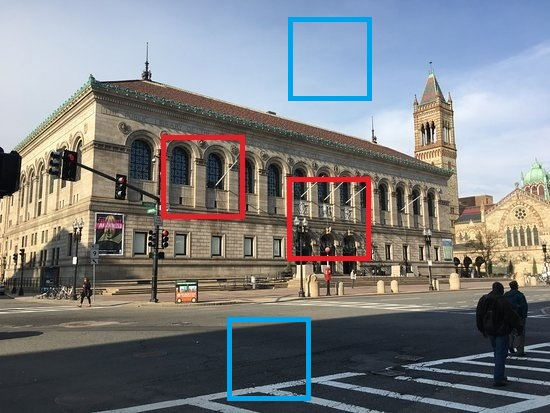
\includegraphics[width=0.41\textwidth]{library}
\\[0.1cm]
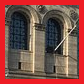
\includegraphics[width=0.1\textwidth]{library_1}

\includegraphics[width=0.1\textwidth]{library_2}
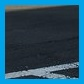
\includegraphics[width=0.1\textwidth]{library_3}

\includegraphics[width=0.1\textwidth]{library_4}
\caption{An example of salient regions and non-salient regions of an image.}
\label{fig:library}
\end{figure}


\section{Background and Related Work}
\subsection{Deep Learning}
\par
Deep learning is a technique which has been applied in the field of artificial intelligence, especially computer vision. It extract features of materials(usually images or videos) by learning deep neural networks. A lot of previous approaches have successfully utilized deep learning on the task of object recognition~\cite{krizhevsky2012imagenet}, faces recognition~\cite{taigman2014deepface} and place recognition~\cite{zhou2014learning,lin2015learning,Arandjelovic16,workman2015wide,weyand2016planet}. 
\subsection{Image/Video Geo-Localization}
\par
As we have mentioned in Section 1, early work by Hays and Efros~\cite{hays2008im2gps} revealed the feasibility of the image localization task. Zamir and Roshan~\cite{zamir2010accurate} used SIFT descriptors for image localization by voting, and constructed a dataset based on Google Street-View to test the efficiency of the algorithm. Lin et al.~\cite{lin2013cross} proposed the first ground-to-overhead geo-localization method, of which the key idea is to learn the relationship between the ground-level images and their over-head appearances. After that, Lin et al.~\cite{lin2015learning} then published an approach by CNN to learn deep representations for ground-to-overhead geo-localization. Vo and Hays~\cite{vo2016localizing} then explored several deep CNN architectures for the cross-domain matching and improved the accuracy of image geo-localization. What's more, Bansal et al.~\cite{bansal2012ultra} proposed a method to capture the structure of self-similarity of patterns on facades for image geo-localization.
\par
Leung et al.~\cite{leung2008localization} designed a monocular vision based particle filter localization system for urban settings that uses aerial reference map. However, because of the great similarity between the task of image localization and video localization, researchers often treat them as the same task.
\par
Visual place recognition is a similar task of image geo-localization. Arandjelovic et al.~\cite{Arandjelovic16} developed NetVLAD, a CNN architecture of which the main component is the VLAD (``Vectors of Locally Aggregated Descriptors'') layer and got the state-of-the-art performance on two challenging place recognition datasets. 

\subsection{Self-Paced Learning}
\par
In machine learning, a sequence of guadually added training samples~\cite{bengio2009curriculum} is called a curriculum. Inspired by the cognitive process of humans and animals, a straightforward way to generate such a sequence is to add samples based on their ``easiness" to learn. However, such ``easiness" is based on specific problem and hard to generalize. In order to solve this problem, Self-Paced Learning (SPL) was introduced by Kumar et al.~\cite{kumar2010self}, which embeds curriculum designing into model learning. In SPL, the curriculum is gradually generated by the model itself based on what it has learned, and it's also a general implementation for curriculum learning. Following that, several works have improved self-paced learning~\cite{jiang2014easy, tang2012shifting, jiang2014self, jiang2015self}. In this paper, we propose self-paced learning method to automatically estimate the saliency score for each region of a frame.
\subsection{Attention-Based Model}
While attention-based models are widely used in recognition tasks, many recent works show that attention based model can improve the performance of machine learning models~\cite{mnih2014recurrent, zheng2015neural}. The key idea of attention-based model is to add attention information to build a representation. This idea is intuitive. For example, when looking at an image, we human beings often recognize the objects on it and then receive the information from the background, rather than receiving information simultaneously from the foreground objects and background scenes. In our approach, we compute the attention to each region by its saliency. 



\section{Methodology}
Assuming we already have a pre-trained model for place recognition, and our main purpose is to refine the model for better accuracy on the image geo-localization task. For the convenience of expression, let us first introduce some notations in Table~\ref{table:notations}. 
\begin{table}
\begin{center}
\begin{tabular}{|c|p{0.35\textwidth}|}
\hline
$q_i$ & region $i$ in the query image $q$\\[0.2cm]
$d_j$ & region $j$ in the database image $d$\\[0.2cm]
$s(q_i), s(d_j)$ & the saliency of the region $q_i, d_j$, i.e. buildingness in our
task, ranged within $[0,1]$ \\[0.2cm]
$m(q_i, d_j)$ & matching score between region $q_i$ and $d_j$, where the better they match, the lower $m(q_i,d_j)$, since it's calculated by the distance between representing vectors\\[0.2cm]
\hline
\end{tabular}
\end{center}
\caption{Notations used in problem formulation.}
\label{table:notations}
\end{table}
\subsection{Saliency Score Estimation}
\par
As we expressed in Section 1, the basic assumption of our work is that salient regions have stronger ability to indicate the geo-location of an image. A salient region in a query image would match less number of regions than non-salient ones in the database. Therefore, an intuitive idea is to calculate the saliency score following Eq~\eqref{eq-1}.
\begin{equation}
s(q_i) \propto \sum_{d_j \in d, d \in D} m(q_i, d_j)
\label{eq-1}
\end{equation}
where $D$ denotes the set of all database images. Analogously, we can also compute the saliency score of database image regions. In order to normalize the saliency score, we compute $s(q_i)$ by Eq~\eqref{eq-2}.
\begin{equation}
s(q_i) = \frac{\sum_{d_j \in d, d \in D} m(q_i, d_j)}{\sum_{q_k \in Q}\sum_{d_j \in d, d \in D} m(q_k, d_j) + \epsilon}
\label{eq-2}
\end{equation}
where $Q$ denotes the set of all query images, $\epsilon$ is a small constant number that guarantee the denominator would be positive. Both the denominator and numerator would be non-negative since $m(q_i, d_j)$ is calculated by the distance of the two regions in a representing space. 
\subsection{Saliency Guided Image and Video Frame Geo-Localization}
\par
At first, we assume that we already have a pre-trained model for place recognition and denote it as $M$. Inspired by the work of Lin et al.~\cite{lin2015learning}, we refine it by applying constructing a Siamese Network and modify the loss function between two images as following:
\begin{equation}
\label{eq-3}
L_s(q,d,l) = \sum_{q_i\in q} \frac{|q_i|}{|q|}  \frac{|d_j|}{|d|} s(q_i)s(d_j)L(q_i, d_j, l)
\end{equation}
where $q$ is a query image, $d$ is an image in the database, $q_i, d_j$ are subimages of them, $|q|$ is the size of the image $q$, $l\in \{0,1\}$ denotes the label whether the two images are at the same place, $s(q_i)$ and $s(d_j)$ are the saliency scores of $q_i$ and $d_j$, $d_j$ is selected by $d_j = \argmin_{{d'} \in d} ||f(q_i), f({d'})||_2 $, and $L(q_i, d_j, l)$ can be computed with Eq~\eqref{eq-4}.
\begin{equation}
\label{eq-4}
L(q_i, d_j, l)=\frac{1}{2}lD^2 + \frac{1}{2}(1-l)\max(0,m-D^2)
\end{equation}
where $D = ||f(q_i) - f(d_j)||_2$ is the Euclidean Distance of the two subimages in the feature space. In particular, $s(q_i)$ is fixed as well as $s(d_j)$ in this step. 
\subsection{Joint Saliency Estimation and Matching Optimization}
\par
We utilize the saliency score to guide the matching optimization and apply the updated match model to estimate more precise saliency score for each region of images. Namely, we are trying to teach the computer how much attention it need to pay to each region of the image by the saliency score. This can be done by an iteration procedure introduced in Algorithm~\ref{alg:joint}.
\begin{algorithm}
\caption{Joint Saliency Estimation and Matching Optimization}
\label{alg:joint}
\begin{algorithmic}  
\FOR{$q_i\in Q$}
	\STATE{set $s(q_i) = 0.5$}
\ENDFOR
\FOR{$d_i\in D$}
	\STATE{set $s(d_i) = 0.5$}
\ENDFOR
\STATE{set $M$ = initial model}
\FOR{iteration $\leftarrow$ 1 to MAX\_ITER}
	\STATE{Estimate saliency socre with Eq~\eqref{eq-2}}
	\STATE{Optimize $M$ with Eq~\eqref{eq-3}}
\ENDFOR
\end{algorithmic}
\end{algorithm}

\section{Experiments}
\par
In the experiments, we use caffe~\cite{jia2014caffe} as the deep learning framework and VGG-CNN-M~\cite{chatfield2014return} as the pre-trained model $M$ for match. 

\section{Conclusion}
